\documentclass[conference]{IEEEtran}
% If the IEEEtran.cls has not been installed into the LaTeX system files,
% manually specify the path to it.  e.g.
% \documentclass[conference]{./IEEEtran}

% Add and required packages here
\usepackage{graphicx,times,amsmath,fontenc,multirow,url,caption}
% I don't even remember which of these packages are even being used 
% but I dare not remove any in case the entire thing breaks

% To create the author's affliation portion using \thanks
\IEEEoverridecommandlockouts

\begin{document}

% Paper title: keep the \ \\ \LARGE\bf in it to leave enough margin.
\title{\ \\ \LARGE\bf Continuous Action Solutions in the {\itshape Lunar Lander} Problem } 
% TODO - better title

\author{Samuel A. Roberts, Spyridon Samothrakis, Simon M. Lucas}

% Uncomment out the following line for invited papers
%\specialpapernotice{(Invited Paper)}

% Make the title area
\maketitle


\begin{abstract}

% come back to this after the rest of the paper's done

\end{abstract}

% No keywords




\section{Introduction}

This paper describes an investigation into solving a continuous problem based on a familiar arcade game, {\itshape Lunar Lander}.

% TODO - actually determine what the core essence of what it is we're doing here before writing the introduction

\section{Motivation}

% TODO - THIS SECTION COULD DO WITH SOME FLESHING OUT

% building upon previous work in MCTS but using a continuous action space?

\subsection{Solving Continuous Problems with Continuous Actions} % this title is awful and it needs changing

Previous research into using MCTS to provide solutions for continuous physics-based problems have examined cases such as the Physical Travelling Salesman Problem \cite{perez14}. Within these continuous contexts, discrete actions have proven to be quite effective, especially with use of macro-actions and some degree of higher level planning \cite{powley12}.  % this section seems clunky

{\itshape Lunar Lander} is an excellent test case to study for many reasons, due to its inherently multi-objective nature. With the objectives to both land quickly while also minimising velocity changes, which cost fuel which must be conserved, it has been an interesting scenario to examine the properties and constraints imposed just by the environment alone. While there have been attempts to solve this deceptively complex problem before using discrete macro-actions \cite{roberts13}, in this paper the problem is being approached as one that can be better solved with continuous actions.


% TODO: this feels unfinished and only barely scratching the surface

% must find more examples of relevant previous research

\section{Methodology}

\subsection{Software Implementation}

% TODO

% anything notable to mention? section worth keeping?

\subsection{Environment and Physics}

% this is a heavily cut down rewritten version of the physics described in sam's 2013 cig paper
% more detail will be added depending on if it is appropriate or not

\subsubsection{Environmental Properties}

The properties of the base environment of {\itshape Lunar Lander} are that it is frictionless, and that it is a two-dimensional plane with horizontal wrapping. This can also be conceptualised as a cylinder. Anything that passes from the left edge of the playing field moves to the right instantaneously, and vice versa.

The other feature of note is the jagged landscape, a simplistic representation of the noisy, crater-filled lunar landscape the game represents. This landscape is constructed as a series of line segments, with each vertex of the jagged landscape being distributed equally horizontally, and randomly vertically. % unclear?

% TODO: DIAGRAM - jagged lunar landscape might be useful (reuse of old one probably not sufficient)

% not sure how much detail should be gone into here? should just cite generation equations from old paper or copy over??

Each vertex of this landscape is generated sequentially. % INCOMPLETE due to uncertainty listed above


\subsubsection{Spaceship Physics}

The spaceship within this game world is modelled as an a circular mass with some basic physical properties, such as a position within the game world $\boldsymbol {s}$, a velocity $\boldsymbol {v}$, an orientation $\theta$, an angular velocity $\omega$ and a radius of a bounding sphere $r$ used for collision detection with the landscape.

This collision detection method is based on the lowest point of the spaceship's bounding circle coming into intersection with the highest point of the landscape for the line perpendicular between the ship and the bottom of the playing field, as can be seen in Figure \ref{fig:diagram_landscapepoint}.

% this needs a diagram for clarity: reuse the old one? reusing it temporarily
\begin{figure}[hbtp]
\centering
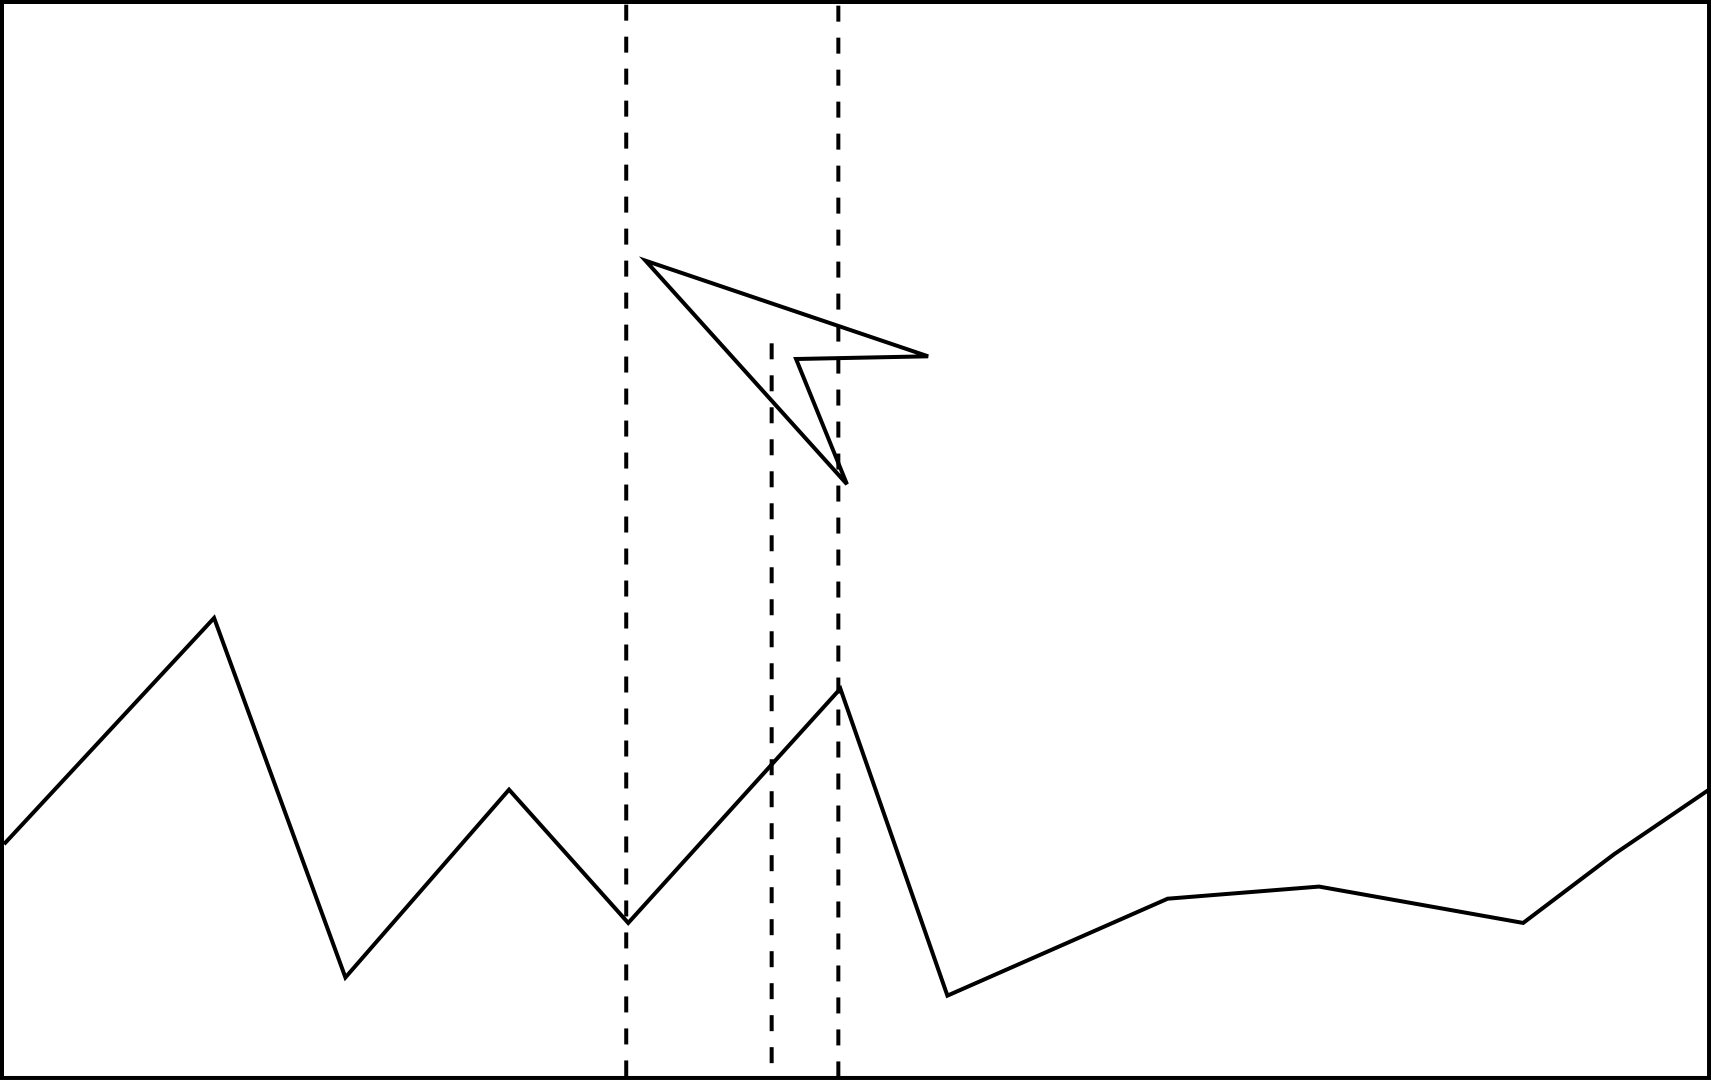
\includegraphics[scale=0.4]{img/landscapepoint}
\caption{The point closest to the spaceship on the landscape lies in between two of the defined vertices of the landscape, and requires interpolation to calculate the y co-ordinate from the x co-ordinate of the ship.}
\label{fig:diagram_landscapepoint}
\end{figure}

As the landscape is stored as a series of line segments, interpolation must be used in the event the ship is not perfectly aligned with one of the landscape axes. The point that lies on the line segment that the ship is being checked against is calculated through simple linear interpolation based on which two vertices the ship is horizontally closest to. For the ship's centre $\boldsymbol {s}$, the left nearest landscape vertex $\boldsymbol {p}^{l}$ and the right nearest landscape vertex $\boldsymbol {p}^{r}$, the point of collision $\boldsymbol {p}^{c}$ against the landscape is calculated as 

% does this constitute self-plaigarism???

\begin{equation}
\boldsymbol {p}_{x}^{c} = \boldsymbol {s}_{x}
\boldsymbol {p}_{y}^{c} = \boldsymbol {p}_{y}^{l} + v(\boldsymbol {p}_{y}^{r} - \boldsymbol {p}_{y}^{l})
\end{equation}

where $v$ is a value between $0$ to $1$ used for interpolation, and can be calculated as follows.

\begin{equation}
v = \frac{ {\boldsymbol {s}_{x} - \boldsymbol {p}_{x}^{l}}}{ {\boldsymbol {p}_{x}^{r} - \boldsymbol {p}_{x}^{l}} }
\end{equation}

Collision is then true if the following statement is true:

\begin{equation}
\boldsymbol {s}_{y} + r \geq \boldsymbol {p}^{c}_{y}
\end{equation}

The ship colliding with the landscape constitutes the end of the {\itshape Lunar Lander} game. The conditions surrounding this collision, including speed, orientation of the ship, and fuel used, constitute whether the nature of the collision is a success or a failure.


\subsection{Continuous Action MCTS} % this can be renamed something much better presumably

\subsubsection{Heuristic} % this too

% TODO - meeting or discussion might be good to be entirely certain on what's going on in the code
% DISCUSS IN MEETING: use of a two-stage approach: might be good to mention this?? temporary holdover?????

\section{Results}

% pending
% DISCUSS IN MEETING: we know that an effective two-stage solution exists, but how can this be written up?
% DISCUSS IN MEETING: the solution works even with noise as well, can the amount of time taken to reach the landing pad be improved?
% DISCUSS IN MEETING: is there any useful information to report, tables, graphs, etc? my methodology is too empirical, can't think of a better way of discussing results without graphs and tables
% DISCUSS IN MEETING: any alternate approaches feasible to compare against?

\section{Conclusion}

% pending
% DISCUSS IN MEETING: this entire section
 
% Use \section* for the acknowledgments
\section*{Acknowledgements}
Samuel Roberts is supported by an EPSRC PhD Studentship.
% any other acknowledgements??

\bibliographystyle{IEEEtran}
\bibliography{lunarcontbib}
\end{document}